\documentclass[conference]{sig-alternate}

\usepackage[tight,footnotesize]{subfigure}
\usepackage{algorithm}
\usepackage{algorithmic}
\usepackage{times}
\usepackage{graphics}
\usepackage{graphicx}
\usepackage{epstopdf}
%\usepackage{slashbox}

\usepackage{epsfig}
\usepackage{amstext}
\usepackage{amssymb}
\usepackage{amsmath}
\usepackage{url}
\usepackage{psfrag}
\usepackage{verbatim}
\usepackage{color}
%\usepackage{hyperref}
\usepackage[bf]{caption}

\newtheorem{lemma}{Lemma}
\newtheorem{theorem}{Theorem}
\newtheorem{proposition}{Proposition}
\newtheorem{conjecture}{Conjecture}
\newtheorem{definition}{Definition}

\newcommand {\bear}{\begin{eqnarray}}
\newcommand {\eear}{\end{eqnarray}}
\newcommand {\bearn}{\begin{eqnarray*}}
\newcommand {\eearn}{\end{eqnarray*}}
\newcommand {\barr}{\begin{array}}
\newcommand {\earr}{\end{array}}
\newcommand {\done} {\hfill\quad\vrule height4pt WIDTH4PT}
\def\cee#1#2{\left(\barr{c} #1\\ #2 \earr \right)}
\def\tA{\tilde{A}}
\def\tL{\tilde{L}}
\def\tM{\tilde{M}}
\def\tP{\tilde{P}}
\def\real{{\rm I\!R}}
\def\cS{{\cal S}}
\def\cF{{\cal F}}
\def\hT{\hat{T}}
\def\b1{\mathbf{1}}
%\def\hr{\hat{R}}
%\def\RR{\mathbb{R}}


\newcommand{\la}{\lambda}
\newcommand{\al}{\alpha}
\newcommand{\be}{\begin{equation}}
\newcommand{\ee}{\end{equation}}
\newcommand{\bi}{\begin{itemize}}
\newcommand{\ei}{\end{itemize}}
\def\bearn{\begin{eqnarray*}}
\def\eearn{\end{eqnarray*}}
\def\bheader#1{\noindent{\bf #1}}
\def\bie#1{\item{\bf{#1}}}

\newcommand{\bmax}{\mathop{\boldsymbol{\max}}}
\newcommand{\bmin}{\mathop{\boldsymbol{\min}}}
\newcommand{\bargmax}{\mathop{\mathbf{argmax}}}
\newcommand{\bargmin}{\mathop{\mathbf{argmin}}}

%%%%%%%%%%%%%%%from harald
\newcommand{\hide}[1]{}

\newcommand{\fix}{\marginpar{FIX}}
\newcommand{\new}{\marginpar{NEW}}
\newcommand{\RR}{\mathbb{R}}
\newcommand{\NN}{\mathbb{N}}
\newcommand{\tr}{{\rm tr}}
\newcommand{\tU}{P}
\newcommand{\tV}{Q}
\newcommand{\tW}{{\tilde{W}}}
\newcommand{\tR}{{\tilde{R}}}
\newcommand{\ba}{{\bf a}}
\newcommand{\bb}{{\bf b}}
\newcommand{\bd}{{\bf d}}
\newcommand{\identity}{I}
\newcommand{\ones}{{1\!\!1}}
\newcommand{\elprod}{\otimes}
\newcommand{\WMW}{{\rm WMW}}
\newcommand{\stepfct}{{\bf 1}}
\newcommand{\hy}{\hat{Y}}
\newcommand{\hr}{\hat{R}}
\newcommand{\rimp}{R^{\rm o\& i}}
\newcommand{\rank}{{\rm Rank}}
\newcommand{\nrank}{{\rm Nrank}}
\newcommand{\anr}{{\rm ANR}}
\newcommand{\aanr}{{\rm A}^{\rm 2}{\rm NR}}
\newcommand{\pr}{ \bar{R}}
\newcommand{\rmse}{{\rm RMSE}}
\newcommand{\Robs}{R^{\rm obs}}
\newcommand{\topk}{{\rm TOPK}}
\newcommand{\areatop}{{\rm ATOP}}
\newcommand{\ppp}{{\rm Prec}_u @ }
\newcommand{\rrr}{{\rm Rec}_u @ }
\newcommand{\sN}{\tilde{N}}
\newcommand{\mult}{} %\cdot
\newcommand{\auc}{{\rm AUC}} %\cdot
\newcommand{\gauss}{{\cal N}} %\cdot
\newcommand{\Qi}{i} %\cdot
\newcommand{\hQ}{\hat{Q}} %\cdot
\newcommand{\hP}{\hat{P}} %\cdot
\newcommand{\hM}{\hat{M}} %\cdot
\newcommand{\precision}{{\rm P}} %\cdot
\newcommand{\recall}{{\rm R}} %\cdot
\newcommand{\ndcg}{{\rm nDCG}} %\cdot
\newcommand{\dcg}{{\rm DCG}} %\cdot
\newcommand{\sdcg}{{\rm sDCG}} %\cdot
\newcommand{\err}{{\rm ERR}} %\cdot
\newcommand{\map}{{\rm MAP}} %\cdot
\newcommand{\popcount}{{\rm pop}} %\cdot
\newcommand{\countall}{{\rm \# ratings}} %\cdot
\newcommand{\hitrate}{{\rm HR}} %\cdot
\newcommand{\ic}{i_0} %number of items
\newcommand{\uc}{u_0} %number of users
\newcommand{\jc}{j_0} %rank of low-rank MF, or latent dimensions


\newcommand{\cc}{CircleCon} %rank of low-rank MF, or latent dimensions
\newcommand{\com}[1]{{\color{red}\bf #1}}
\newcommand{\ci}{{\cal C}}
\newcommand{\cat}{{\rm cat}}

%%%----------------------- make it tighter ----------------------------
%\topskip -0.5in            %between header and text
%\parskip 0in            %gap between paragraphs
%\floatsep 0.1in           %space left between floats
%\textfloatsep 0.1in       %space between last top float or first bottom float and the text
%\intextsep 0.1in          %space left on top and bottom of an in-text float
%\dblfloatsep 0.1in        %floatsep for 2 column
%\dbltextfloatsep 0.05in    %space between last top float or first bottom float and the text
%\abovecaptionskip 0.01in   %space above caption
%\belowcaptionskip 0.02in   %space below caption
%\abovedisplayskip 0.1in   %space before maths
%\belowdisplayskip 0.1in   %space after maths
%\arraycolsep 0in       %gap between columns of an array
%\topsep 0in             %space between first list item and preceding paragraph.
%\partopsep 0.1in          %extra space added to \topsep when environment

%\ifCLASSINFOpdf
%  \graphicspath{{./fig/}}
%\else
%\fi

%\hyphenation{op-tical net-works semi-conduc-tor}

\begin{document}
%\conferenceinfo{CoNEXT'12,} {December 10--13, 2012, Nice, France.}
%\CopyrightYear{2012}
%\crdata{978-1-4503-1775-7/12/12}
%\clubpenalty=10000
%\widowpenalty = 10000

\title{Multipath IP transmission: Motivation, Design, Performance}
%\author{
%\alignauthor Guibin Tian and Yong Liu\\
%        \affaddr{Department of Electrical and Computer Engineering}\\
%        \affaddr{New York University Polytechnic School of Engineering}\\
%        \affaddr{Brooklyn, NY, USA 11201}\\
%        \email{gt680@nyu.edu, yongliu@poly.edu}
%}



\maketitle


\begin{abstract}
%\boldmath
Multipath Internet transmission has become available in recent years. Most devices have more than one interfaces that can be connected to Internet. Especially the booming of mobile devices introduces the greatest chance for multipath communication. 

In $2011$, multipath TCP was introduced as RFC by IETF. This draft defines the architecture and guideline of multipath TCP development. Also, a popular multipath TCP implementation\cite{mptcp} has been in process for several years. Most research work on multipath TCP is based on this implementation. But, as the name refers, multipath TCP is only designed for TCP traffic. Inside the current Internet infrastructure, it is still an accepted assumption that most Internet traffic is transmitted via the TCP protocol. However, the rise of new streaming applications and P$2$P protocols that try to avoid traffic shaping techniques will likely increase the use of other protocols like UDP as a transport protocol.

In this paper, we introduce multipath communication at network layer instead of transmission layer. By implementing multipath feature at network layer, almost all traffic on Internet can enjoy the convenience and performance improvement introduced by multipath. Also, because of the design and internal characters of multipath TCP and multipath IP, we can get a lighter weight implementation of multipath at network layer. We implement our proposition in the latest Linux kernel and evaluate its performance under multiple Internet scenarios. 

\end{abstract}

%\category{H.5.1}{Information Systems}{Multimedia Information Systems}[Video(e.g., tape, disk, DVI)]
%\terms{Design}
%\keywords{Adaptation, DASH, Emulab, Multiple CDN, SVR}
%\IEEEpeerreviewmaketitle

%!TEX root =conext14.tex
\section{Introduction}
\label{sec:intro}
Multipath has become available in recent years. Also, IETF proposed RFC $6182$ specifically for multipath TCP development in $2011$. By introducing multipath between both ends for one connection, not only higher throughput can be achieve, different characters on different paths can be complementary to satisfy different user requirement under volatile Internet congestion situations.

In data center network, almost every two nodes are connected by multiple physical paths. Because of this unique structure, multipath has been deployed for a long time to increase throughput and improve reliability.

Most current devices (Mainly mobile devices) have more than one internet interface ($3$G, WiFi), it is possible to make use of this facility to improve internet transmission. In use cases that end users want high throughput, like user is watching HD movies, parallel multipath transmission can greatly improve throughput. In use cases that end users have intermittent internet connection on one interface, multipath connection can provide smooth switching between connections which improves user experience.	


Current work on multipath is mainly on TCP. In multipath TCP, if the user has more than one internet interface, there will be more than one sub TCP sub-flow in one TCP connection. In this way, the user does not need to re-establish the connection again when switching connection. The most popular implementation is from \cite{mptcp}, which maintains multiple sub-flows for a single TCP connection. But in multipath TCP also has some problems. 

\begin{enumerate}
\item In multipath TCP, between the client and server, there will be multiple TCP connections. Normally, the number of connections is all the possible composition of all interfaces between the client and server. If clients and the server both have 2 interfaces, it means that there will be 4 sub-flows for each connection. This can be a very high workload for the server if the server has large number of parallel clients.

\item In multipath TCP, each sub-flow has its own congestion window, and also, to guarantee 
fairness, the congestion windows of all sub-flows are coupled. This makes the mechanism too complicated.

\item In multipath TCP, as designed, there will be two levels of sequence number. There will be a mapping between the overall sequence number and independent sequence number of each sub-flow. Also, this will make things complicated. Complicated things are always vulnerable.

\item In multipath TCP, when switching connection, TCP slow-start will be done which may result in delays.

\item multipath TCP can only be used in TCP connection. For other transport layer protocol, multipath can not be used. Although TCP traffic is dominating the Internet nowadays, there are studies showing that other protocols like UDP still play important roles. For some specific applications, TCP is not the best choice. 
\end{enumerate}

Based on this, we propose our multipath implementation at IP layer.

Implementing multipath functionality at IP layer has following pros.
\begin{enumerate}
\item IP layer is relatively simpler than transport layer because it is connectionless. We do not need to deal with the complicated congestion window and flow control which resides in TCP protocol. Instead, we only do the implementation at IP layer and the implementation is also connectionless. This is totally transparent to other layers. 

\item More straightforward to implement multipath at IP layer since multipath is in fact multiple IP addresses.

\item MPTCP can only be used for TCP connection while MPIP is eligible for all protocols above IP layer.
\end{enumerate}

Our contribution is four-fold.
\begin{enumerate}
\item We propose the overall design and architecture of multipath IP transmission. By comparing our design with multipath TCP, we see that implementing multipath at IP layer has lighter weight than at TCP layer because of the internal simple character of IP layer.

\item We implement our design in the latest Linux kernel. 

\item We evaluate our implementation in different Internet environments. We show that our implementation can match multipath TCP in TCP protocol, and also, other protocols like UDP can fit perfectly with multipath IP.
\end{enumerate}

The rest of the paper is organized as follows. Section \ref{sec:related} describes the related work.
The design of our implementation is introduced in Section \ref{sec:design}. In Section \ref{sec:evaluation}, we report the experimental results for our multipath IP design. We conclude the paper with summary and future work in Section \ref{sec:conclusion}.

%!TEX root =conext14.tex
\section{Related Work}
\label{sec:related}
todo...
%!TEX root =conext14.tex
\section{Design of MPIP}
\label{sec:design}
Based on Linux kernel $3.12$, we implement our prototype in Ubuntu. Most work resides in the IP layer with some compatibility modification in other modules. Also, the addition of multipath IP feature is transparent to users, a.k.a, all user\textquoteright s applications won\textquoteright t be modified.

The framework of MPIP is shown in Figure~\ref{fig.arch}. 
\begin{figure}
\centering
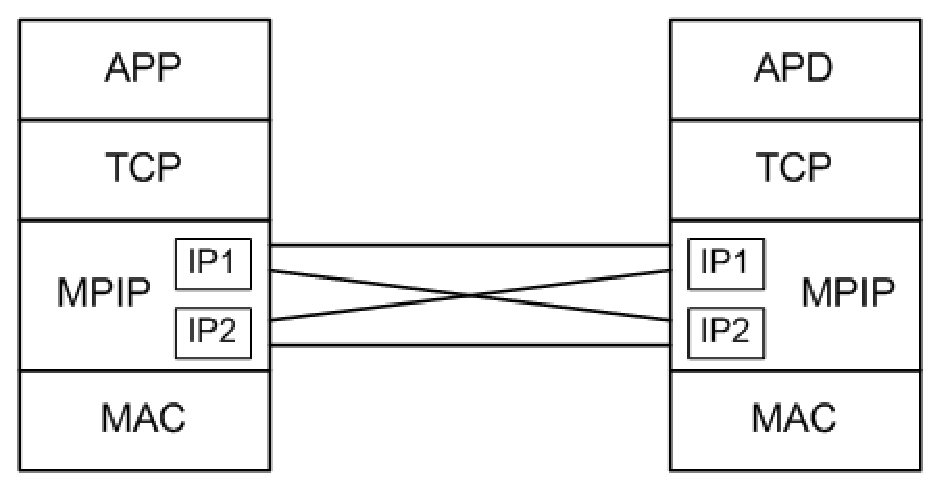
\includegraphics[width=0.8\linewidth]{fig/arch.eps}
\caption{Overall design of MPIP}
\label{fig.arch}
\end{figure}

%\subsection{MPIP Working Modes}
%As we can see, assume there are $M$ and $N$ networking interfaces on each end, there will be $M*N$ available paths totally between the two nodes. Among all the available paths, we can have different modes to make use of them. Generally, there are two modes of MPIP.
%
%\begin{enumerate}
%\item Parallel mode. In parallel mode, all available interfaces will send out packets that are assigned to them. The number of packets that are assigned to them is calculated according to their relative capability. In parallel mode, all available interfaces will be used to transmit packets. There can be two scenarios. If the packet passed down is large enough (larger than some threshold value), the packet will be to be sent out through more than one interface. In this case, one unique token for all fragments, fragmentation offset, and the information about the main IP address will be contained in the options data in the IP header. The receiver will merge all the data together into the packet from the main IP address and pass it to the upper layer. If one of the fragments lost during the transmission, the whole packet will fail after some expiration time. The data size that is assigned to each path is calculated through their capability. If the packet passed down doesn\textquoteright t need any fragmentation because it is a small one, then we need to choose one path to send out the packet. In this case, random number is used to choose the final path according to their capability.
%
%\item Backup mode. In back-up mode, there is only one working interface. Other interfaces will be the backup interfaces which means that the backup interface will take over the connection when the working interface isn\textquoteright t available. In backup mode, that is only the main interface that is used to transmit packets that are passed down from upper layer. If the current working main interface isn\textquoteright t the one when the connection was initiated, MPIP module needs to add the original interface information into the options field of IP header to tell the receiver the destination of this packet. If the current working main interface is the same as the initial one, nothing is going to change. The receiver won\textquoteright t do any additional process for the packet once it receives it, just passes it to the upper layer.
%\end{enumerate}
%
%In both parallel mode and backup mode, there is a main interface which is used to notate the connection. In parallel mode, one main interface is chosen when the application starts the connection. In backup mode, the working interface is the main interface. In both modes, when the main interface isn\textquoteright t available at any time, other interfaces will take over seamless and act as the main interface without being known by upper layers because this main interface is maintained at the transport layer. With this mechanism, all connection won\textquoteright t be re-established after interface switching.

\subsection{NAT consideration}
For each connection, probably there can be multiple NAT devices on the path. In this scenario, we can\textquoteright t only use the exposed IP address as the identification one node, instead, the combination of IP address and port number is unique for each node. So in the following sections, when referring the address of a node, we will use the combination of IP address and port number.


\subsection{IP Layer Control Communication}
As stated before, most implementation is done at IP layer. In the IP layer, everything is like UDP, there is no feedback information at IP layer. The kernel just sends out the packets through a proper path, then all the other things will be dealt with by upper layer. Like in TCP, reliable transmission is guaranteed by its own control protocol.

To support additional multipath feature at IP layer, we need to introduce feedback message at IP layer to enable the peers to talk with each other. Not like in TCP, which has specific control packets like ACK packets to support the protocol, we use piggyback technology to implement the feedback message in IP layer. This can avoid excessive control packets and reduce overhead of the MPIP.

For each MPIP enabled packet that goes out of the system, we add an additional data block at the end of user data. As shown in Figure~\ref{fig.cm}.

%\begin{figure}
%\centering
%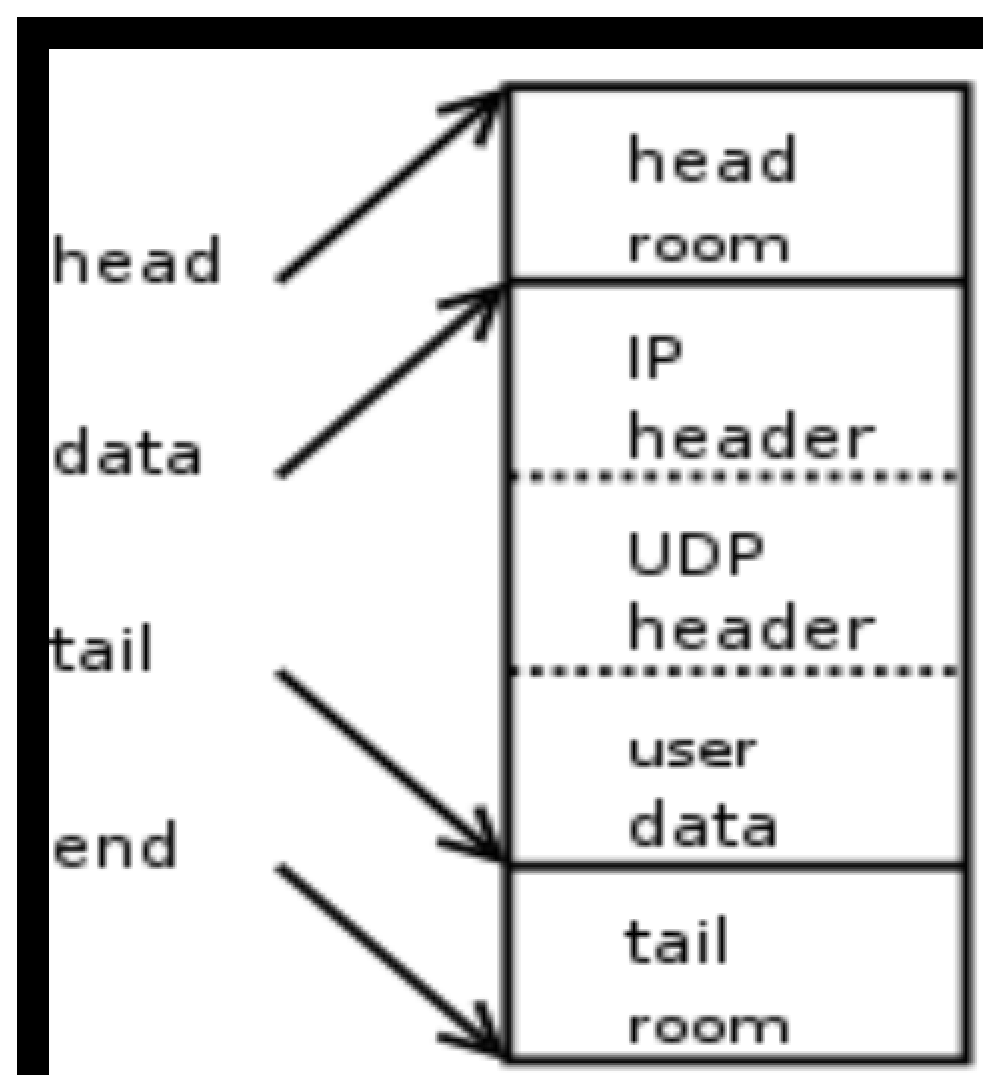
\includegraphics[width=0.8\linewidth]{fig/cm.eps}
%\caption{CM data block}
%\label{fig.cm}
%\end{figure}

\begin{table}
\caption{\label{tb.cm}Control Message Structure}
\centering
\begin{tabular}{|c|}
\hline
Control Message \\
\hline
\emph{Node ID,} \\
\emph{Session ID,} \\
\emph{Path ID,} \\
\emph{Feedback Path ID,} \\
\emph{Packet Timestamp,} \\
\emph{Path Delay}\\
\emph{Local Address List}\\
\emph{CM Flags}\\
\emph{Checksum}\\
\hline
\end{tabular}
\end{table}

The content in the control message is shown in Table~\ref{tb.cm}.

\emph{Node ID} is the globally unique identification of one node. Because IP address can change at different times, we use the MAC address of one of NICs at the local node. When the system starts, we initiate node ID\textquoteright s value with one of the node\textquoteright s NIC card\textquoteright s MAC address and keep it unchanged until the system exits. Every time the node sends out a packet, it fills the field of \emph{node ID} with the previously extracted value into the control message.

\emph{Local Address List} carries all local IP addresses. This list will be used to construct new MPIP paths.

\emph{CM Flags} notates the functionality of the packet. With different value of \emph{CM Flags}, different action will be taken when the packet has been received. 

\emph{Checksum} is used to verify the validation of the CM data block. This value is assigned by simply adding up the value of all other field in the CM data block. This will be recalculated when received to judge whether a CM data block is attached in this packet.

Other fields of the CM block will be explained in following sections.

\subsection{MPIP availability handshake}

As a new feature in Linux, MPIP needs to be backward compatible. For one specific connection, before enabling MPIP functionality, the two sides need to synchronize with each other to make sure both have MPIP feature enabled. Locally, every node maintains Table~\ref{tb.me} to identify the availability of MPIP at its opposite nodes. Before the initial synchronization finishes, all communication on the connection is normal traffic without MPIP enabled.

\begin{table}[htbp]
\caption{\label{tb.me}MPIP availability}
\centering
\begin{tabular}{|c|c|c|c|}
\hline
IP Address & Port Number & MPIP Availability & Query Count\\
\hline
${IP}_{1}$ & ${P}_{1}$ & True  & $2$ \\
\hline
${IP}_{2}$ & ${P}_{2}$ & False & $5$ \\
\hline
\end{tabular}
\end{table}


When a node sends out a packet, it checks locally whether the relative IP address is MPIP enabled in Table~\ref{tb.me}. If not, it 
copies the current packet before sending it out. Besides sending out the original packet, the system inserts the CM block into the copied packet with \emph{CM Flags} of $3$. This value is used for MPIP query. When this packet is received by a MPIP enabled node, the receiver adds the sender into Table~\ref{tb.me}, then sends back the confirmation to the sender with \emph{CM Flags} of $4$. But the time to send back this confirmation message depends on the protocol of the connection, specifically, for TCP and non-TCP, we have different process. 

For any protocol rather than TCP, we populate a new packet, fill all header fields with the correct information, and insert the CM block at the end, then send back to the sender right away. But for TCP, we add the confirmation request into a waiting list, and piggyback the confirmation when next TCP message is sent out to that specific node. There are two reasons to do this different process. 

\begin{enumerate}
\item For protocols rather than TCP, like UDP, because they don't have built-in feedback loop, which means that all traffic can be of only one direction. In this situation, we can't wait until there are packets available to send back 

\item For the protocol of TCP, we don't simply populate a new TCP packet and send back because the sequence numbers of each direction are different. Through our experiments, some NAT devices will refuse to transfer this packet if the sequence number messes up for the same TCP connection. We can manage to maintain the right sequence numbers to fill them into the confirmation packet, but by considering the whole design of our system, we choose to add the request into a waiting list, when there is TCP packet available to send back, we make a copy of the packet and insert the CM block with \emph{CM Flags} of $4$. In this case, there will be two consecutive TCP packets that go through the path with the same sequence number. The NAT devices will simply consider that they are retransmission.
\end{enumerate}

For both the MPIP query packet and MPIP confirmation packet, we populate new packets based on the original packets. These two packets won't be passed to the upper layers because they are generated at the network layer and stop there too, they don't mean anything to upper layers. The network layer drops all MPIP packets with \emph{CM Flags} of $3$ and $4$ after processing them.

With the handshake flow above, the smallest number of query packet that will be sent for the whole process is $1$. But sometimes because of packet loss or synchronization issues, there can be multiple query packet sent out at both ends. This is not a problem because the design of the system allows receiving more than on query packet and send back the confirmation. For nodes that don\textquoteright t support MPIP, we can\textquoteright t send out query messages forever. In Table~\ref{tb.me}, the column \emph{Query Count} maintains how many query messages have been sent out to relative IP addresses. If the number is larger than a threshold value, it assumes that IP address doesn\textquoteright t support MPIP. Considering that packet loss is rare event in Internet nowadays, we set this value to $5$ in our system, this is more than enough to make sure a MPIP enabled node can receive and reply this message with successful transmission. In a connection will only one-way traffic, if the receiver is MPIP enabled while the sender isn't, then no query packet will be sent out at all.

Generally, for MPIP enabled nodes, they can have more than one IP address. In this situation, multiple synchronization messages will be transmitted for the same node.

\begin{figure}
\centering
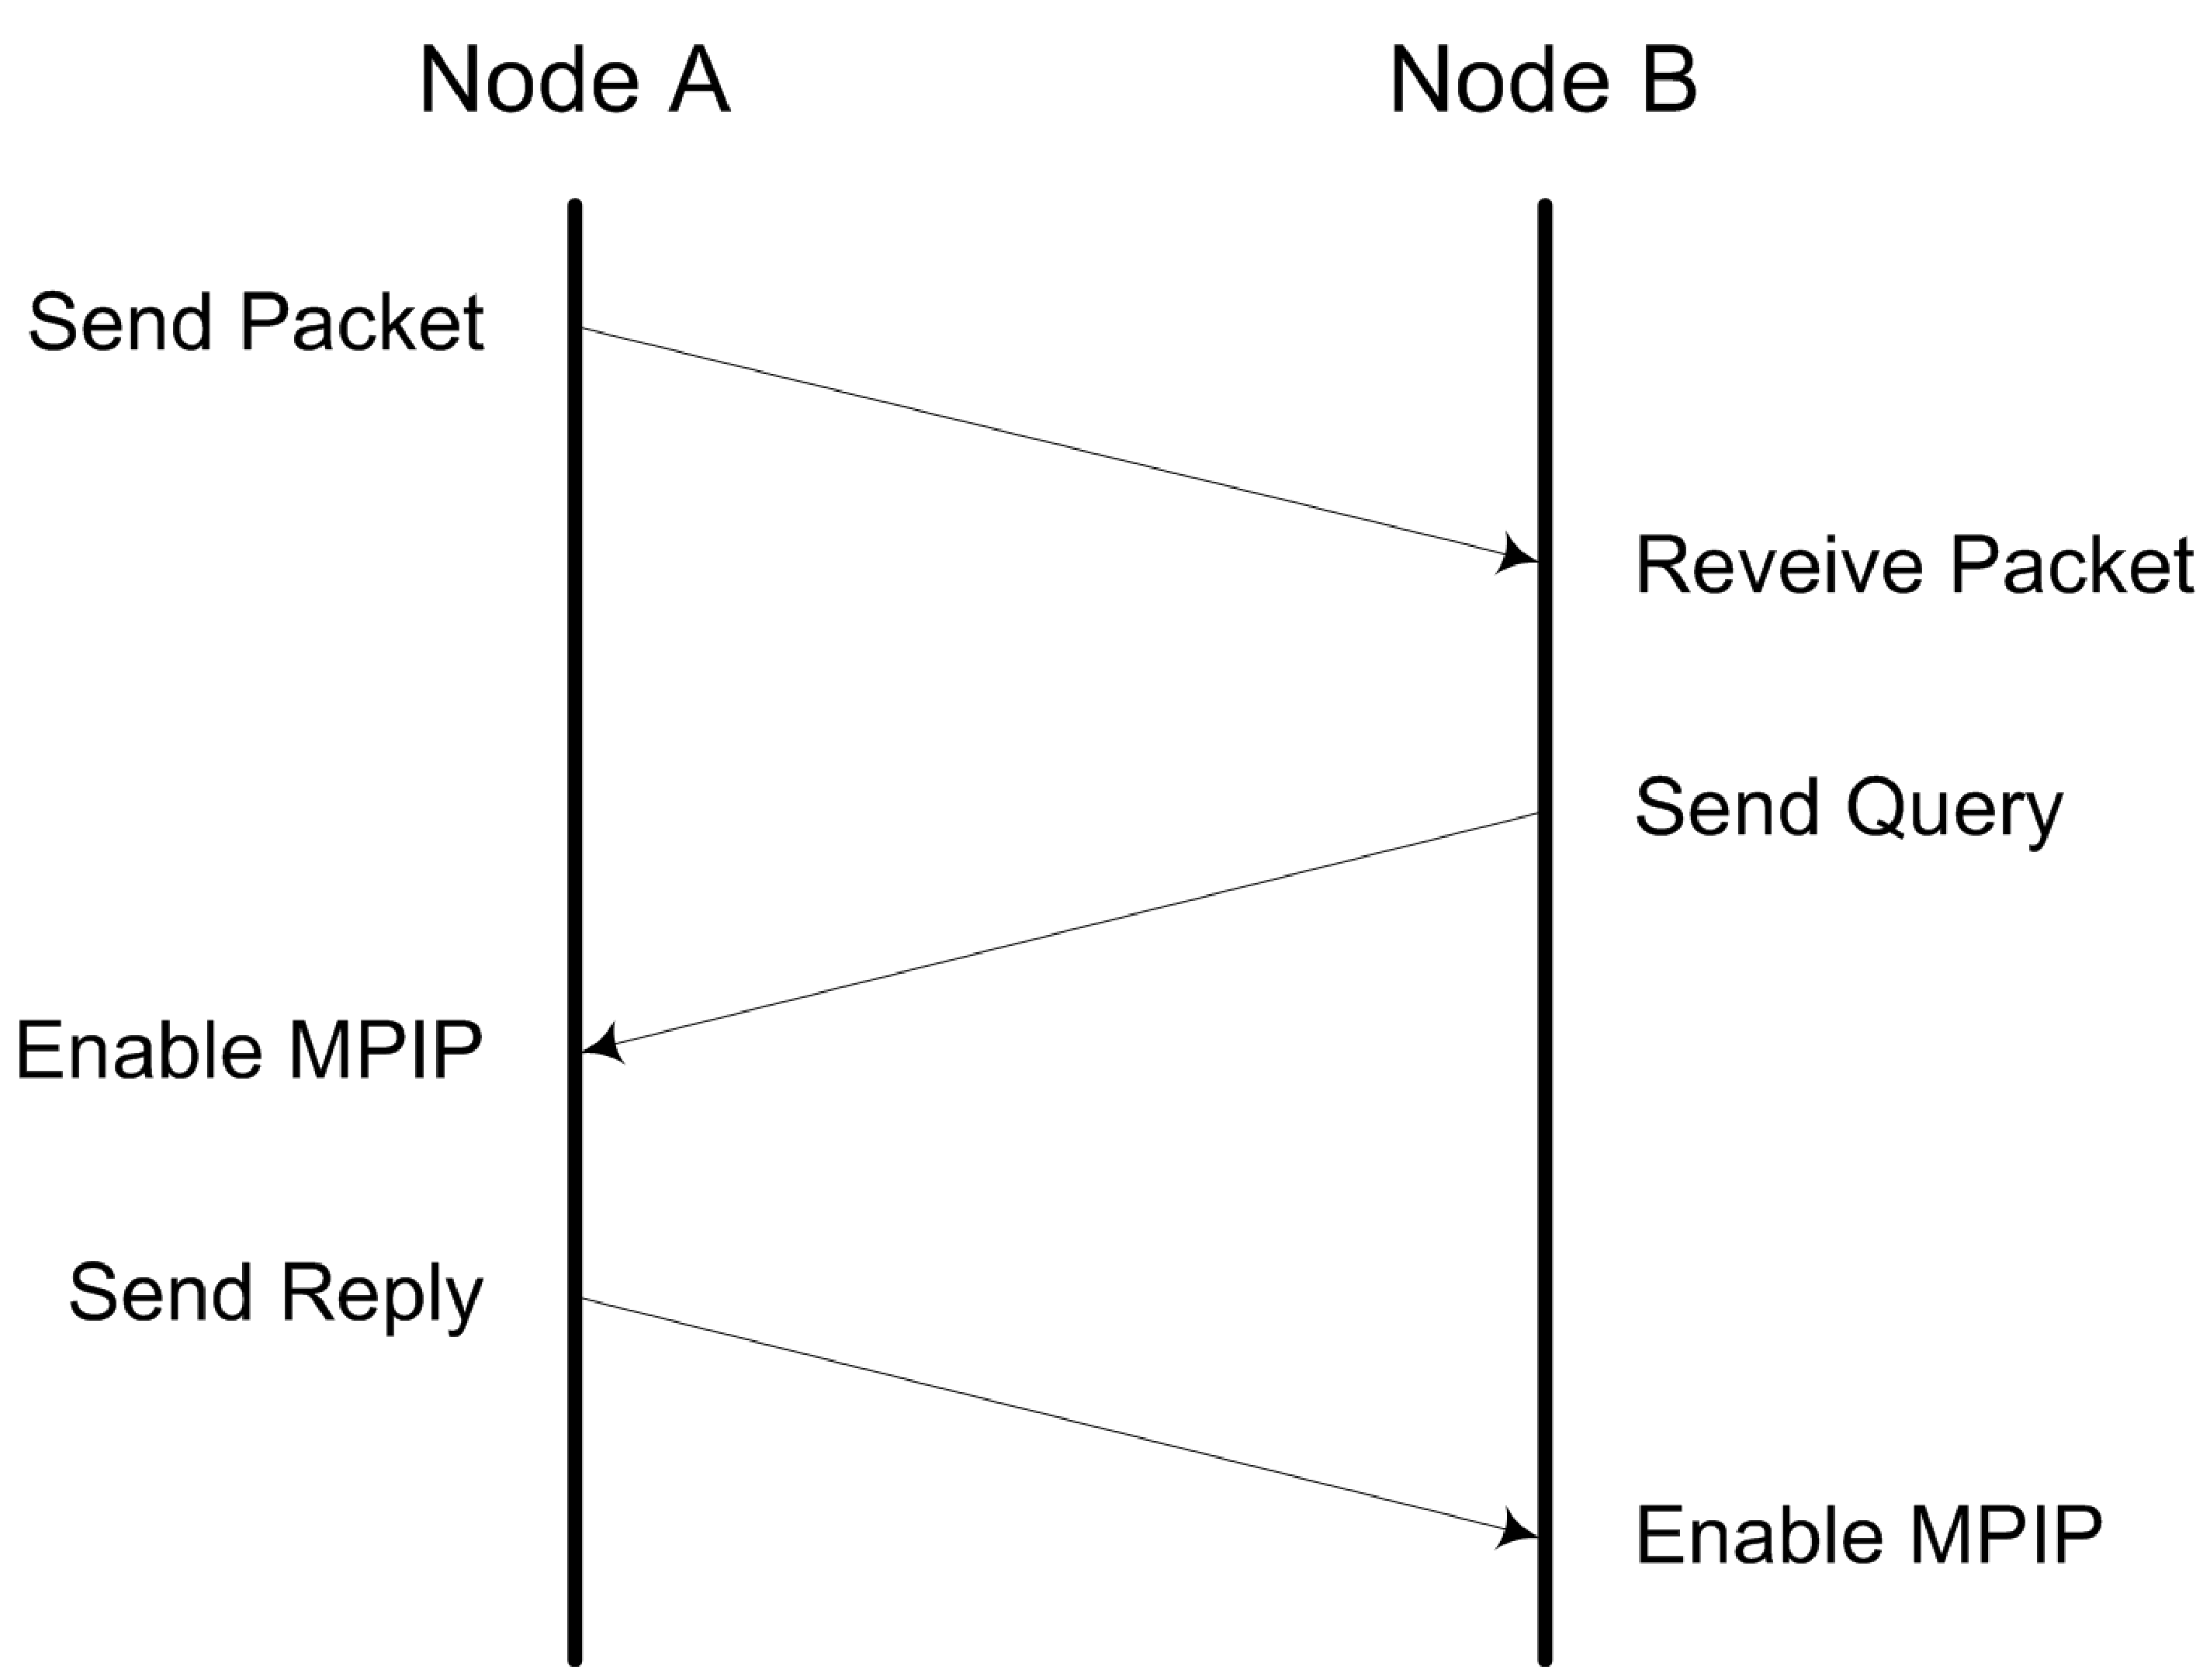
\includegraphics[width=0.8\linewidth]{fig/me.eps}
\caption{MPIP availability synchronization}
\label{fig.me}
\end{figure}

\subsection{Multipath TCP Transmission}
Through our experiments and previous studies\cite{mptcp}, NAT devices have a lot of interference to end-to-end connections, especially for TCP packets. The most straightforward limitation for TCP packets is that many NAT devices will drop TCP packets that don't have a connection related to them. This means that if we transmit TCP traffic on a path rather than the original one, the NAT devices on the path will probably drop these packets before they arrive at the destination. There is no such problem in Multipath TCP\cite{mptcp} because MPTCP has a totally independent TCP connection on each path which will pass this category of NAT devices successfully. In our MPIP implementation, we provide two options to solve this problem.

\subsubsection{Fake TCP connection}
In NAT devices that drop TCP packets without relative connection information, we cheat them by constructing fake TCP connections on relative paths. The construction of TCP contains three-way handshakes. Instead of constructing real TCP connections, we implement a simple three-way handshake at network layer which is similar as TCP handshake, but it only happens at network layer. 

As shown in Table~\ref{tb.cm}, the field \emph{Local Address List} carries all local IP addresses. When the client receives the IP address list of the server, it extracts its own IP address list, then sends out a SYN packet through each possible path to the server except the original one which is the one that was used to initiate the connection. When the server receives this SYN packet, it replies with a SYN-ACK packet through the same path. After the client sends out the final ACK packet to the server, the three-way handshake for our fake TCP connection is completed successfully, then this path will be used to transmit MPIP TCP packet without being dropped. The whole process only happens at network layer, all packets for the three-way handshake have \emph{CM Flags} value of $5$, they will be dropped after being processed at network layer. By having fake TCP connections, we can make use of multiple feature for TCP traffic without the overhead of managing multiple TCP connections as in MPTCP.

\subsubsection{UDP wrapper}
The other option we provide for multipath TCP traffic is UDP wrapper. Because there is no connection information in an UDP packet, most NAT devices don't have limitation on regular UDP traffic. We can make use of this feature to wrap our TCP packet with a UDP packet to pass the NAT devices and unwrap it when received.

As shown in Figure~\ref{fig.udpwrapper}, at the sender side, every time the network layer gets a TCP packet from transport layer, the system chooses a path to send the packet out as shown in Section~\ref{sec:path}. If the chosen path isn't the original path, we wrap the user data and TCP header into an UDP packet.

%\begin{figure}
%\centering
%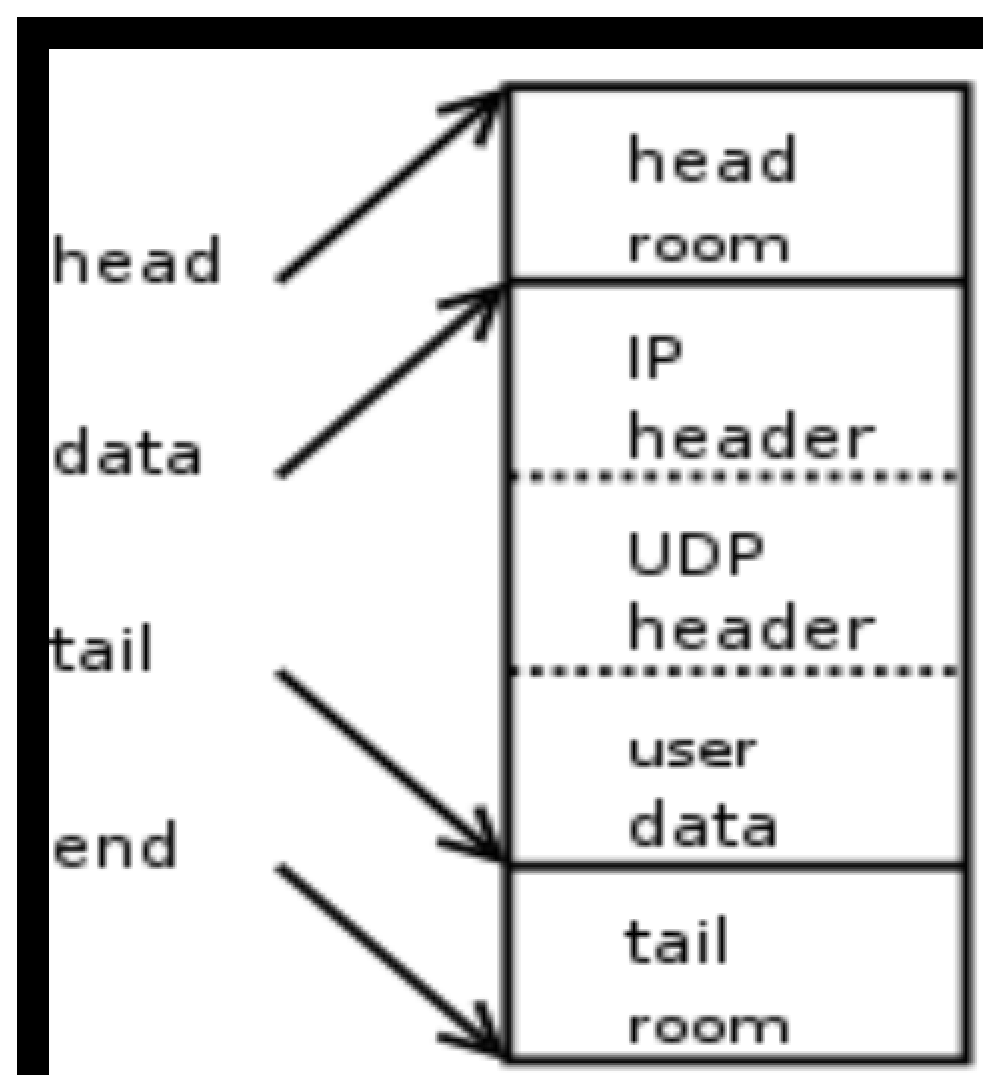
\includegraphics[width=0.8\linewidth]{fig/cm.eps}
%\caption{UDP wrapper for TCP packet}
%\label{fig.udpwrapper}
%\end{figure}

\subsection{Path Management}
\label{sec:path}

As shown in Figure~\ref{fig.arch}, given $M$ and $N$ interfaces at each end, there are totally $M*N$ possible paths on the connection. On each end of one connection, the same number of paths with the opposite direction will be maintained.

\subsubsection{Delay-Based Solution}

When the system tries to send a packet, it will have to choose the most suitable one among all the available paths. To achieve this goal, we need to have some parameters to notate the capability of each path. Generally, there are two ways to notate the character of one path, the first is loss based and the second is delay based. Nowadays, packet losses in networks are rare events, this makes loss rate estimation is difficult and coarse in accuracy. But delay estimation can be accurate enough with a proper measurement.

For network delay, it consists of following $4$ parts.

\begin{enumerate}
\item Processing delay. Time routers take to process the packet header
\item Queuing delay. Time the packet spends in routing queues
\item Transmission delay. Time it takes to push the packet onto the link
\item Propagation delay. Time for a signal to reach its destination
\end{enumerate}

Among the $4$ parts above, processing delay, transmission delay and propagation delay are fixed value for one path, they can be treated as constant $C$. But for queuing delay $Q$, it will change as the traffic that passes through the router changes. igure~\ref{fig.delay} shows the trend of network delay as of the traffic on the path changes.

\begin{figure}
\centering
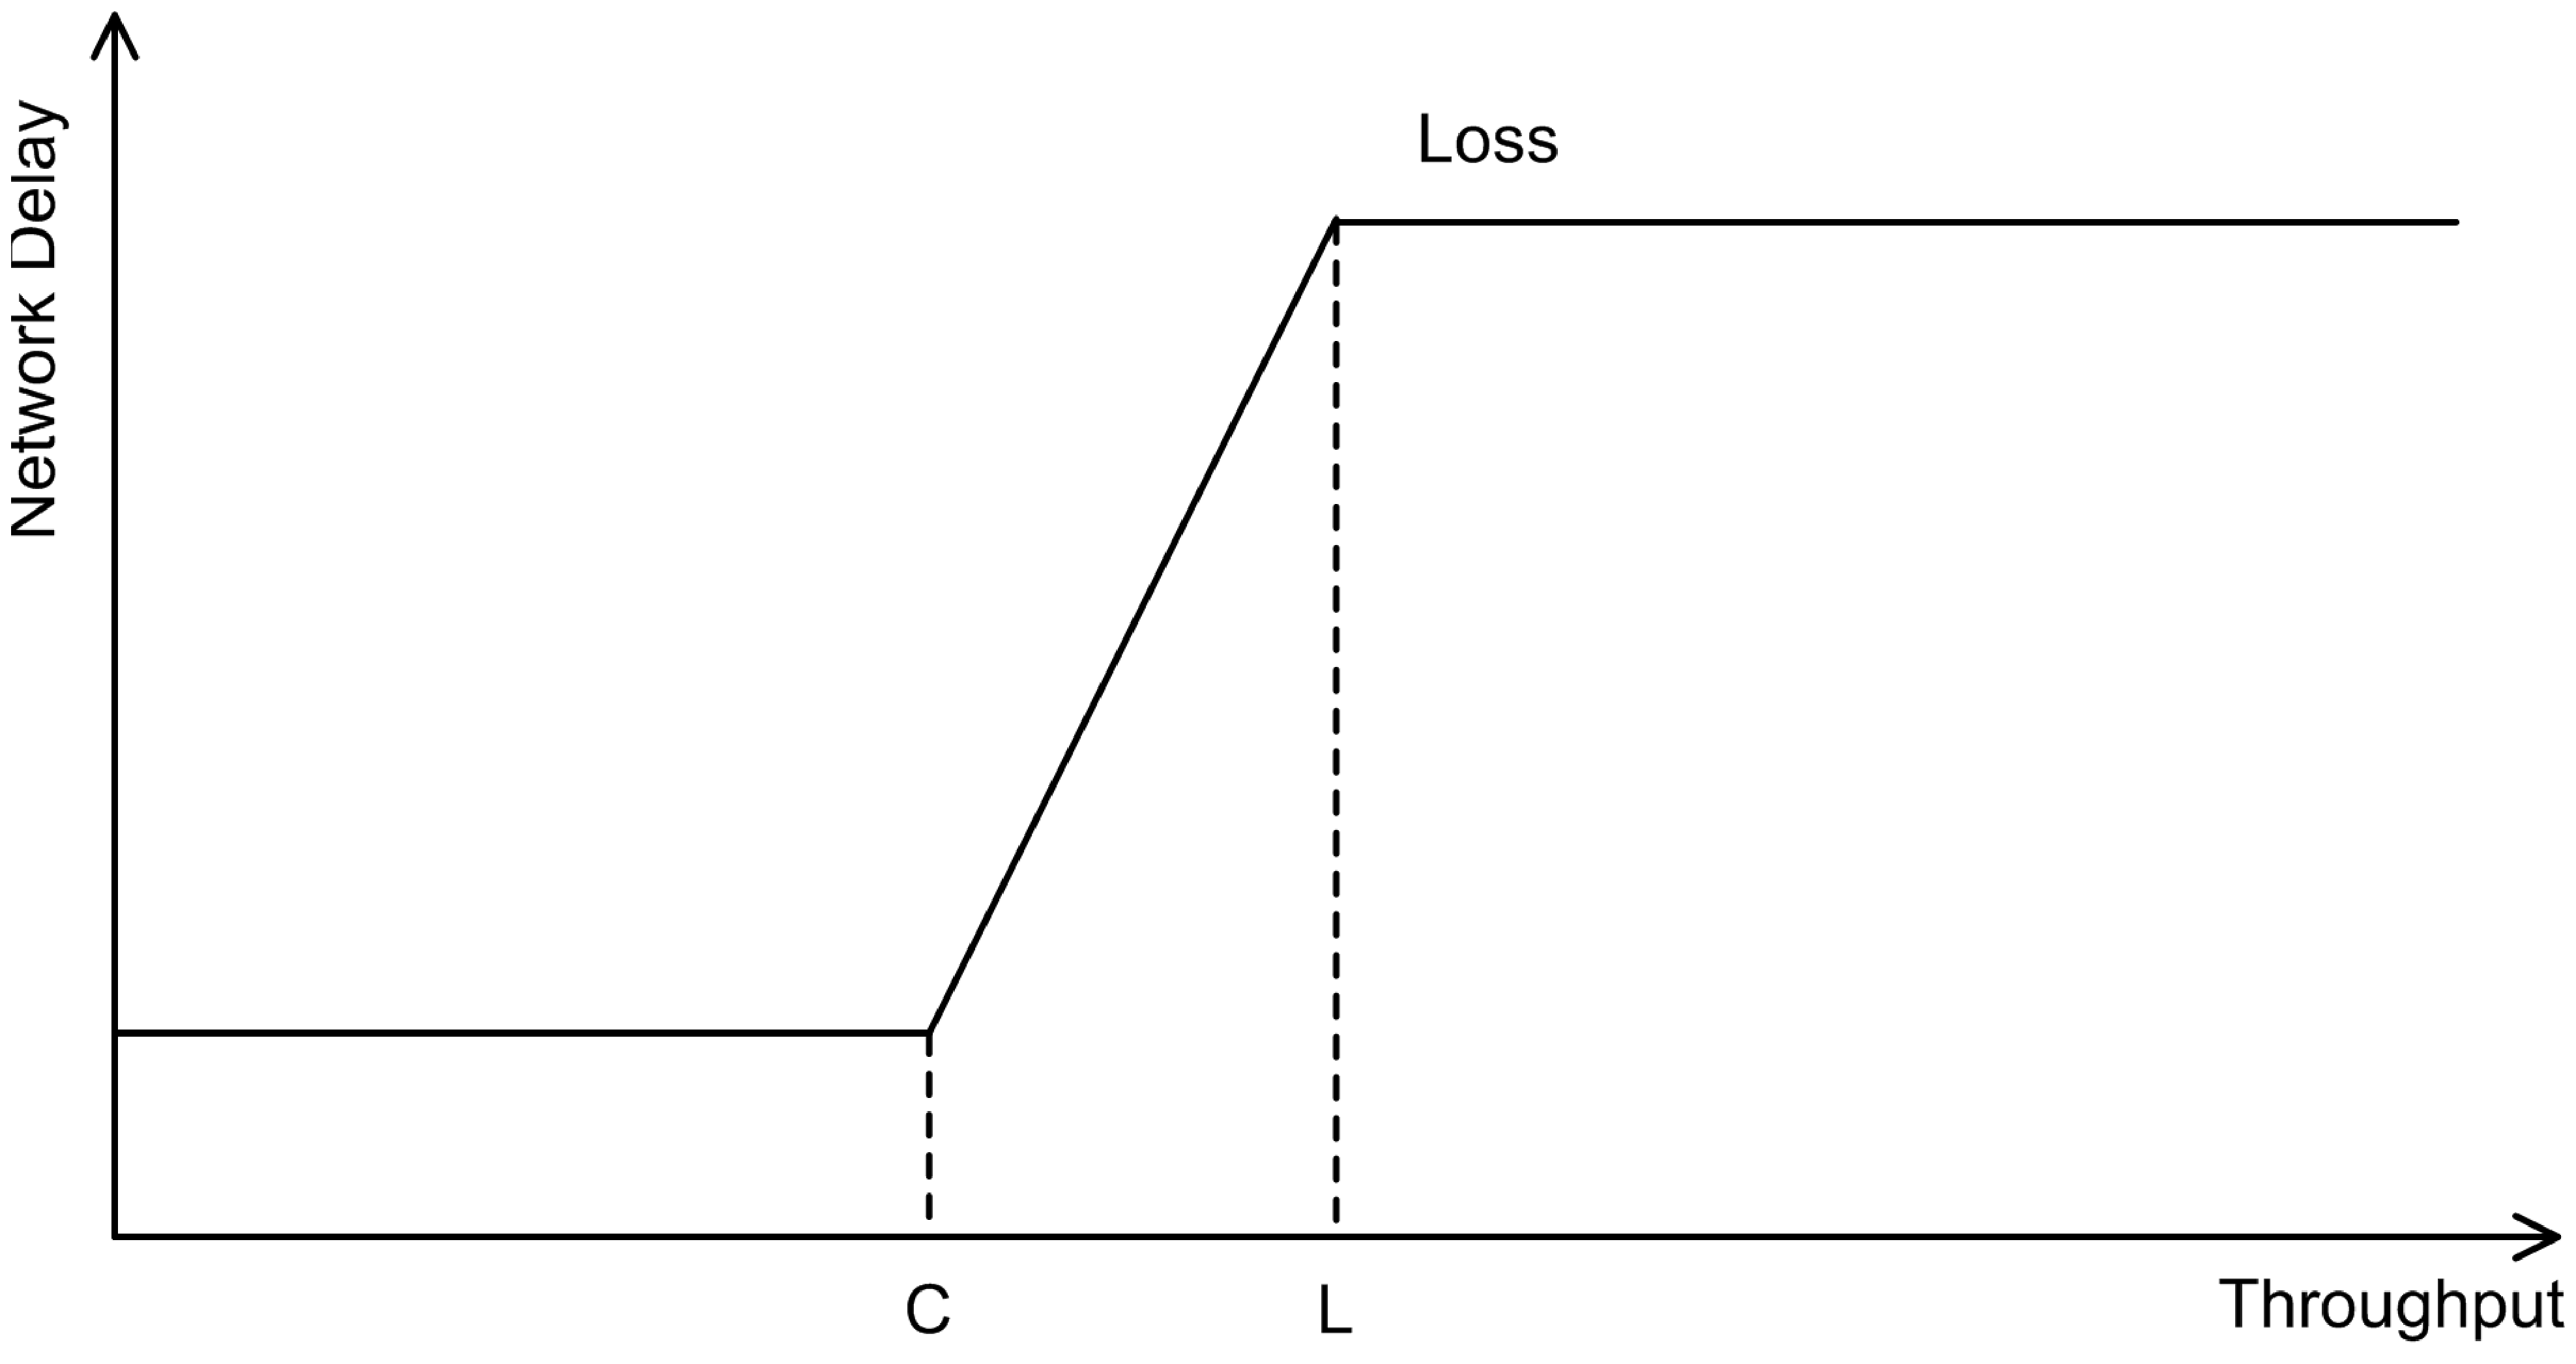
\includegraphics[width=0.8\linewidth]{fig/delay.eps}
\caption{Network delay trend as throughput increases}
\label{fig.delay}
\end{figure}

We can see that the queue in the router starts to accumulate at point $C$, but still, there is no loss. Starting from point $L$, the queue size overflows. The minimum and maximum network delay for the path can be measured at point $C$ and point $L$. By comparing the real-time delay with minimum and maximum network delay, we can deduce the remaining capability of the path, and do relative adjustment of the characters.


\subsubsection{Path Maintenance}

In our system, we maintain all available paths through Table~\ref{tb.pi}.

\begin{table*}
\small
\caption{\label{tb.pi}Path information}
\centering
\begin{tabular}{|c|c|c|c|c|c|c|c|c|c|c|c|c|}
\hline
Node &  Path & Session & Src &   Src & Dest & Dest &   Minimum       & Real-Time      & Real-Time      & Maximum       & Path    & Feedback\\
 ID  &   ID  & ID & IP  &  Port &  IP  & Port &  Network Delay  & Network Delay  & Queuing Delay  & Queuing Delay & Weight  & Time\\
\hline
$ID$&${PID}_{11}$&${SID}_{1}$&${SIP}_{1}$&${SP}_{1}$&${DIP}_{1}$&${DP}_{1}$&${D_{min}}_{11}$&$D_{11}$&${Q}_{11}$&${{Q}_{max}}_{11}$&$W_{11}$&$T_{11}$ \\
\hline
$ID$&${PID}_{12}$&${SID}_{1}$&${SIP}_{1}$&${SP}_{1}$&${DIP}_{1}$&${DP}_{2}$&${D_{min}}_{12}$&$D_{12}$&${Q}_{12}$&${{Q}_{max}}_{12}$&$W_{12}$&$T_{12}$ \\
\hline
$ID$&${PID}_{21}$&${SID}_{2}$&${SIP}_{1}$&${SP}_{2}$&${DIP}_{1}$&${DP}_{1}$&${D_{min}}_{21}$&$D_{21}$&${Q}_{21}$&${{Q}_{max}}_{21}$&$W_{21}$&$T_{21}$ \\
\hline
$ID$&${PID}_{22}$&${SID}_{2}$&${SIP}_{1}$&${SP}_{2}$&${DIP}_{1}$&${DP}_{2}$&${D_{min}}_{22}$&$D_{22}$&${Q}_{22}$&${{Q}_{max}}_{22}$&$W_{12}$&$T_{22}$ \\
\hline
\end{tabular}
\end{table*}

Node ID is used to identify the sender globally. In all packets sent out from this node, the same value will be filled into the field of \emph{node ID}.

Path ID is used to identify one path. It is maintained at each end, we set it as locally unique Arab numbers starting from $1$. This value is generated only when adding new paths into Table~\ref{tb.pi}. 

Because of NAT mapping, the same node can have different IP address and port number that will be seen on the other side at different time or for different application. That's why the column \emph{Session ID} needs to be added into Table~\ref{tb.pi}. When sending out one packet, the final path will only be chosen from the ones that have the correct session id. The detail of session is explained in Section~\ref{sec:session}. Here we just consider a session is the synonym of one connection.

As the names show, source IP, source port, destination IP and destination port show the address information of the path. Because of the existence of NAT devices, IP address is not enough to identify the address information. Also, the IP addresses can be different on the two nodes even if they represent the same physical path because NAT devices change IP addresses. For the same pair of nodes, one instance of Table~\ref{tb.pi} is maintained at each side, the IP addresses here are the addresses that are seen by the node that maintain the instance of Table~\ref{tb.pi}.

Initially, Table~\ref{tb.pi} is empty. Every time one new combination of IP address and port number is flagged as MPIP enabled in Table~\ref{tb.me}, it adds new paths to the table with every available local IP address, and the value of Node ID is extracted from Table~\ref{tb.wi} which is maintained to conveniently map node ID with IP address and port number. 

Structure of Table~\ref{tb.wi} is very simple, it contains all working IP addresses and port number of one specific node ID. When paths in Table~\ref{tb.pi} are obsolete and need to be removed, relative entries in Table~\ref{tb.wi} will also be removed.

\begin{table}[htbp]
\caption{\label{tb.wi}Node ID vs IP address and Port}
\centering
\begin{tabular}{|c|c|c|}
\hline
 Node ID  & IP Address & Port Number\\
\hline
${ID}_{1}$&${IP}_{11}$&${P}_{11}$ \\
\hline
${ID}_{1}$&${IP}_{12}$&${P}_{12}$ \\
\hline
${ID}_{2}$&${IP}_{21}$&${P}_{21}$ \\
\hline
${ID}_{2}$&${IP}_{22}$&${P}_{22}$ \\
\hline
\end{tabular}
\end{table}


\subsubsection{Feedback Loop}

Unlike multipath TCP, which has built-in congestion control algorithms, in the Network layer, to be able to detect the capability of each path, we need some kind of feedback information like in TCP. But we don\textquoteright t need the same complicated congestion control algorithms. Instead, we just roughly estimate capability of each path to make a choice.

In Table~\ref{tb.pi}, all fields referring to network delay will be filled or calculated by feedback information. In Table~\ref{tb.cm}, the fields \emph{Path ID} and \emph{Packet Timestamp} are used to measure network delay. When a node A sends out a packet, it chooses a path from Table~\ref{tb.pi}, fill the field \emph{Path ID} in control message with the chosen path ID, also, get the current time with system\textquoteright s jiffies value and fill the filed \emph{Packet Timestamp} in control message. After the receiver node B receives this packet, it updates records in Table~\ref{tb.ps}. The receiver extracts node ID path ID and timestamp from the control message. The node ID and path ID are directly used to identify records in Table~\ref{tb.ps}, for the timestamp $T_1$, the receiver calculate the timestamp $T_2$ with its local jiffies value and uses $T_2-T_1$ as the one way delay from node A to node B. Node B checks whether the path that identified by the node ID and path ID already exists in Table~\ref{tb.ps}, if yes, it updates the path\textquoteright s delay with $T_2-T_1$, otherwise, it adds a new record into Table~\ref{tb.ps}.

\begin{table}[htbp]
\caption{\label{tb.ps}Path Feedback information}
\centering
\begin{tabular}{|c|c|c|c|c|c|}
\hline
 Node   & Path    & Path      & Feedback           \\
  ID    &  ID     & Delay     & Time               \\
\hline
${ID}_{11}$&${PID}_{11}$&${D}_{11}$&${J}_{11}$   \\
\hline
${ID}_{12}$&${PID}_{12}$&${D}_{12}$&${J}_{12}$   \\
\hline
${ID}_{21}$&${PID}_{21}$&${D}_{21}$&${J}_{21}$   \\
\hline
${ID}_{22}$&${PID}_{22}$&${D}_{22}$&${J}_{22}$   \\
\hline
\end{tabular}
\end{table}

In practice, the value of path delay calculated here isn\textquoteright t the real delay value because of time difference between node A and node B, even, it can be negative. But as we will see later, time difference between A and B doesn\textquoteright t have any influence on our algorithm.

When node B needs to send packet back to node A, it chooses the record with the earliest feedback time in Table~\ref{tb.ps}, it fills the field \emph{Feedback Path ID} and \emph{Path Delay} of the control message with relative value in Table~\ref{tb.ps}, and updates the column \emph{Feedback Time} with system\textquoteright s current jiffies value. When node A receives this packet, it extracts the path ID and path delay value in the control message, and fills the path delay value into the column \emph{Real-Time Network Delay} in Table~\ref{tb.pi}. To avoid outliers, the value of path delay is calculated by moving average algorithm. At meantime, the column \emph{Feedback Time} is updated with the current local jiffies value.

In practice, IP addresses of devices can be removed or added dynamically. Especially for mobile device, it can connect to different access points(WiFi hotspot/Cellular Tower) at different time, during this stage, its IP address can be changed, removed or added dynamically. Under this situation, the system supports addition and removal of paths from Table~\ref{tb.pi}.

There are two scenarios that new paths will be added into Table~\ref{tb.pi}. The first scenario is when new packets are received, new paths will be added as narrated above. The second scenario is when new IP addresses are assigned to the device, the system will check Table~\ref{tb.pi} to added new path entries for all destination IP addresses. Every time the system sends out packets, it checks the value of the column \emph{Feedback Time} in Table~\ref{tb.pi}, if the the latest update time for the path has exceeds a threshold value, then the system considers the path to be obsolete and remove the path from Table~\ref{tb.pi}. Also, if there are changes of IP addresses locally, like up/down of NICs and change of IP address, there will also be addition and removal of paths.

If there is any changes of local IP addresses, when sending out packets, the value of \emph{CM Flags} in CM block will be $1$ to notify the other node to make changes to relative tables.

In Table~\ref{tb.pi}, except the column \emph{Real-Time Network Delay}, other three delay related columns are calculated through this column.

\begin{enumerate}
\item \textbf{Minimum Network Delay $D_{min}$}. Every time one node receives update of network delay, it update this column with the minimum of its current value and the new real-time network delay.
\item \textbf{Real-Time Queuing Delay $Q$}. According to Figure~\ref{fig.delay}, the value of queuing delay is calculated as $Q=D-D_{min}$ which is the difference between real-time network delay and minimum network delay.
\item \textbf{Maximum Queuing Delay $Q_{max}$}. Maximum queuing delay is updated once the real-time queuing delay $Q$ is larger than $Q_{max}$. When packet loss happens, this value notates the curve section after point $L$ in Figure~\ref{fig.delay}.
\end{enumerate}


\subsubsection{Periodical Heartbeat}

For protocols like TCP, during the whole lifetime of the connection, both sides are sending packets to each other at a high frequency, then at both sides, column \emph{Feedback Time} of Table~\ref{tb.pi} can be updated way before the path becomes obsolete. But there are protocols that don\textquoteright t have this built-in feedback mechanism, like UDP. In some UDP applications, all traffic is one way, there aren\textquoteright t any acknowledgements, which means that the sender can\textquoteright t get feedback information through piggybacked control messages. Under this situation, the sender won\textquoteright t be able to properly add new entries into Table~\ref{tb.pi}, then multipath feature can\textquoteright t be applied at all. 

To solve this problem, in our system, we add periodical heartbeat message on one connection. At each side, when the node receives packets, the system checks Table~\ref{tb.ps} for the specific node, if it finds that the entry with the earliest feedback time is close to the obsolete value, it makes a copy of the received packet, switches the source/destination address information, and sends back the packet with CM block attached. The path to send this heartbeat message will be chosen through the same algorithm as regular IP packet as in Section~\ref{sec:selection}. Through the heartbeat message, we can effectively maintain the active paths between two nodes, and safely remove obsolete paths from Table~\ref{tb.pi}. 

All heartbeat packets have value $2$ for \emph{CM Flags} in the CM block. These packets will be dropped after being processed at network layer.


\subsubsection{Path Selection}
\label{sec:selection}

Every time one node needs to send out packets, it chooses the most suitable path from Table~\ref{tb.pi}. As mentioned above, the candidate paths should have the correction session id for the target connection. The criterion of choosing the best path is on the column of \emph{Path Weight}. Given certain values of the is column for each path, we don\textquoteright t simply choose the path that has the largest path weight which may overuse the path and starve other paths at meantime, instead, we choose the path by random number. For one specific path $k$, the probability $P$ it will be chosen is calculated in Equation~\ref{eq.choose}. By balancing the percentage of packets on each path, system fluctuation can be effectively avoided.

\be
\label{eq.choose}
P(k) = \frac{W_k}{\sum_{i=1}^{N}W_i}
\ee

From above, the path weight is the only criterion to choose the most suitable path, so the calculation of path weight $W$ is critical to the performance of the system. Wrong decision can result in catastrophic disaster. In our prototype, the value of $W$ is calculated by Equation~\ref{eq.bw}. 

In Equation~\ref{eq.bw}, we update the path weight by progressive increasing to make the trend of path weight smooth. The increment consists of two parts. In the first part, we calculate the weight with queuing delay. This is beneficial for high bandwidth-delay product links according to \cite{mptcp}. By assigning high priority for this part, we can achieve high throughput. In the second part, we calculate the weight with the total network delay. For applications that prefer low delay to high throughput, assigning high priority to the second part will be of much benefit. The constant $C_1$ and $C_2$ can be used to adjust the weight of each part.

$SI_q$ and $SI_d$ are the smooth index of queuing delay $Q$ and network delay $D$ of all paths calculated in Equation~\ref{eq.siq}  and Equation~\ref{eq.sid} where $N$ is the total number of paths in Table~\ref{tb.pi}. Please be noted that $Q_{max}$, $Q_{min}$ mean the maximum and minimum queuing delay out of all paths, while $D_{max}$, $D_{min}$ mean the maximum and minimum network delay in Equation~\ref{eq.bw}, Equation~\ref{eq.siq} and Equation~\ref{eq.sid}.
%
%\begin{eqnarray}
%p'(4, 2, S_{4}) &=& \left. \frac{c_{c}(S_{4})}{4} + w(1 - \min(1, \frac{2}{12})2\rho(4))\right. \nonumber \\
%&=& \left. \frac{c_{c}(S_{4})}{4} + w(1 - \frac{1}{3}\rho(4))\right. \label{schemeINotGroup4PeersPeer4}
%\end{eqnarray}

\begin{eqnarray}
\label{eq.bw}
W(k+1) = W(k) + \frac{Q_{max}(k)}{\frac{Q(k)-Q_{min}(k)}{SI_q(k)*C_1}+1} \nonumber \\
\left.		  + \frac{D_{max}(k)}{\frac{D(k)-D_{min}(k)}{SI_d(k)*C_2}+1}\right. 
\end{eqnarray}

\be
\label{eq.siq}
SI_q(k) = 100*(1-\frac{1}{N-1}\sum_{i=k-N+1}^{k-1}\frac{|Q(i) - Q(i-1)|}{Q_{max}})
\ee

\be
\label{eq.sid}
SI_d(k) = 100*(1-\frac{1}{N-1}\sum_{i=k-N+1}^{k-1}\frac{|D(i) - D(i-1)|}{D_{max}})
\ee

Here we only explain the first part of Equation~\ref{eq.bw}, because the second part is almost the same.

Given the path that has the minimum queuing delay $Q_{min}$, we calculate the difference of queuing delay of all paths with $Q_{min}$, and the path weight increases progressively with the inverse ratio of the difference. To avoid divide-by-zero error, factor $1$ is added to the difference.

From Equation~\ref{eq.siq}, the calculated smooth index $SI_q$ is between $0$ and $100$, larger value of $SI_q$ means smoother queuing delay array which means that the current congestion status of each path is more similar, then it is safer to add larger weight value to each path. In the case of small $SI_q$, then congestion of each path has large variation, we need to take extra care to avoid fluctuations, so we reduce the added weight to each path.

Because Linux kernel doesn\textquoteright t have good support of floating point calculation, $Q_{max}$ is set as the denominator to make sure denominator is larger than numerator to avoid zero increment. When the largest path weight in Tabel~\ref{tb.pi} hits a threshold value, all weight values will be normalized to the threshold value.

For each path, when it is added into Table~\ref{tb.pi}, the same initial value will be assigned, after the system has achieved stability, each path will have a proper path weight value that reflects its capability. 

%As shown in Figure~\ref{fig.weight}.
%
%\begin{figure}
%\centering
%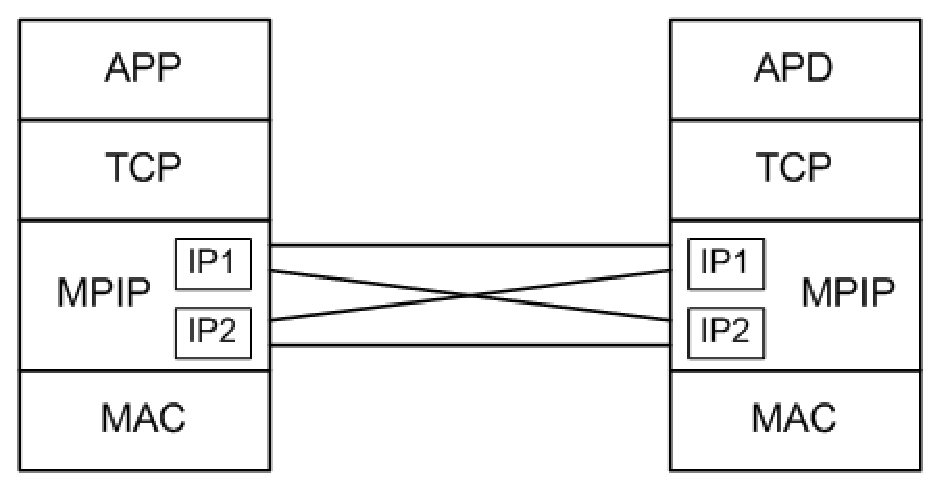
\includegraphics[width=1\linewidth]{fig/arch.eps}
%\caption{Path weight trend for each path}
%\label{fig.weight}
%\end{figure}


\subsection{Session Management}
\label{sec:session}

For one specific connection, it can be identified by a socket at each end.  Each socket pair is described by a unique $4$-tuple consisting of source and destination IP addresses and port numbers of local and remote socket addresses. In our prototype, we call a connection\textquoteright s unique socket a session. Since multiple IP paths is introduced into the system, a session module is development to manage the mapping between different IP addresses and session. To maintain all sessions, each MPIP enabled node will maintain an instance of Table~\ref{tb.ss}.

\begin{table*}
\caption{\label{tb.ss}Session Information}
\centering
\begin{tabular}{|c|c|c|c|c|c|c|c|c|c|}
\hline
Node  & Session &  Source &  Source & Destination & Destination & Update  & Protocol  &    Next      \\
  ID  &   ID    &    IP   &   Port  &     IP      &    Port     &  Time   &           &  Sequence No \\
\hline
${ID}_1$&${SID}_1$&${SIP}_{1}$&${SPORT}_{1}$&${DIP}_{1}$&${DPORT}_{1}$&$T_1$&TCP&$S_1$               \\
\hline
${ID}_1$&${SID}_2$&${SIP}_{1}$&${SPORT}_{2}$&${DIP}_{1}$&${DPORT}_{2}$&$T_2$&UDP&$0$                 \\
\hline
${ID}_2$&${SID}_1$&${SIP}_{2}$&${SPORT}_{3}$&${DIP}_{2}$&${DPORT}_{3}$&$T_3$&TCP&$S_2$              \\
\hline
${ID}_2$&${SID}_2$&${SIP}_{2}$&${SPORT}_{4}$&${DIP}_{2}$&${DPORT}_{4}$&$T_4$&UDP&$0$                 \\
\hline
\end{tabular}
\end{table*}


\subsubsection{Addition/Removal of Sessions}

Session ID is the unique identity of one session in local system, but globally, it still needs node ID to identify the node it belongs to. From Table~\ref{tb.ss}, we can see that different nodes can have the same session ID. Same as path ID, session ID is Arab numbers starting from $1$. This value is generated only when adding new sessions into Table~\ref{tb.ss}. At both sides of one connection, the session ID needs to be the same to locate the correct entry in Table~\ref{tb.ss}.

After the MPIP availability handshake has been successfully completed on one connection, when sending out a packet, the sender checks Table~\ref{tb.ss} to see whether a proper session entry has been generated, if not, one new record will be added with an unique session id. Until now, no other paths have added into Table~\ref{tb.pi} for this session because there was no session id. We extract the IP addresses, port numbers and protocol from packet headers, and gets the destination node ID from Table~\ref{tb.wi}, then it generates a new session ID and adds one new entry into Table~\ref{tb.ss}. The receiver extracts these information and inserts one entry into its own Table~\ref{tb.ss}. For the same session, both sides of the connection have the same session id.

Now, both sides of the connection has the entry that identify the same session. Besides the session ID, all IP addresses and port numbers can be different because of NAT devices, but this doesn\textquoteright t have a problem because the IP addresses and port numbers only need to be the values that are seen locally.

Removal of sessions is decided by expiration. At each node, every time it sends or receives a non-heartbeat packet, it will go to Table~\ref{tb.ss} to get the session ID to fill the control message, meantime, it updates the column \emph{Update Time}. For an active session, this time stamp should be updated frequently. If the timesstamp expires a threshold value, the session is considered to be obsolete and removed from Table~\ref{tb.ss}.

Session entries won\textquoteright t be modified after they have been added into Table~\ref{tb.ss} even the IP address that initiates the session doesn\textquoteright t exist any more. The only operation that can apply to them is removal. 

Once session entry has been inserted into Table~\ref{tb.ss} at both side, different paths can be chosen to transmit future packets that belong to this session. For each connection, the system internally maintains a socket pair with source/destination IP addresses and ports, the system maintained socket information is the same as the pair maintained in Table~\ref{tb.ss}. 

\subsubsection{Workflow of Sending/Receiving Packets}

For one regular packet, when being sent, it goes through application layer, transportation layer, then arrives at network layer which is IP layer. Before the packet arrives at IP layer, socket information inside the packet is the one that stores in a system maintained table. In regular scenario, the system will find a proper interface to push out the packet according to the destination IP address in the IP header and routing table. But since we need to apply MPIP, additional operations need to be done after the packet arrives.

When sending a packet, the system looks into Table~\ref{tb.ss}, and finds the session entry that matches the original socket information, extracts the session ID to fill into the field \emph{Session ID} in the control message. To choose the proper path to send out the packet, the first thing is to locate which paths in Table~\ref{tb.pi} are eligible for this connection. Given the destination IP address in the socket pair, we can find the \emph{Node ID} in Table~\ref{tb.wi}, then in Table~\ref{tb.pi}, all entries that have the correct node ID are eligible. Among all these paths, the most suitable path will be chosen out through the mechanism introduced in Section~\ref{sec:path}. 

The chosen path\textquoteright s path ID will be assigned to the field \emph{Path ID} in the control message for delay measurement at the receiver as narrated above. Meantime, we modify the source and destination IP address in the IP header with the chosen path\textquoteright s source and destination IP address. Then we route the packet with the new IP header information to a proper interface.

When receiving a packet, the receiver extract the node ID and session ID in the control message, with these two parameters, the node locates the original socket pair in Table~\ref{tb.ss}, and modify the IP header with source and destination IP address, modify TCP header with source and destination port. For the fields related to path measurement, they will be processed as explained int Section~\ref{sec:path}. Now the packet is back to it shape that can be recognized by upper layer, it is ready to be pushed up.

If UDP wrapper is used to transmit TCP traffic, when receiving one packet, we are capable to know this UDP packet is a wrapper for a TCP packet instead of a regular UDP packet by checking the column \emph{Protocol} in Table~\ref{tb.ss}. After removing the UDP wrapper, socket information will be extracted from Table~\ref{tb.ss} and filled into the TCP and IP header. The protocol field of IP header needs to be modified to TCP too.

%The whole process of the sending and receiving packets is shown in Figure~\ref{fig.flow}.
%
%\begin{figure}
%\centering
%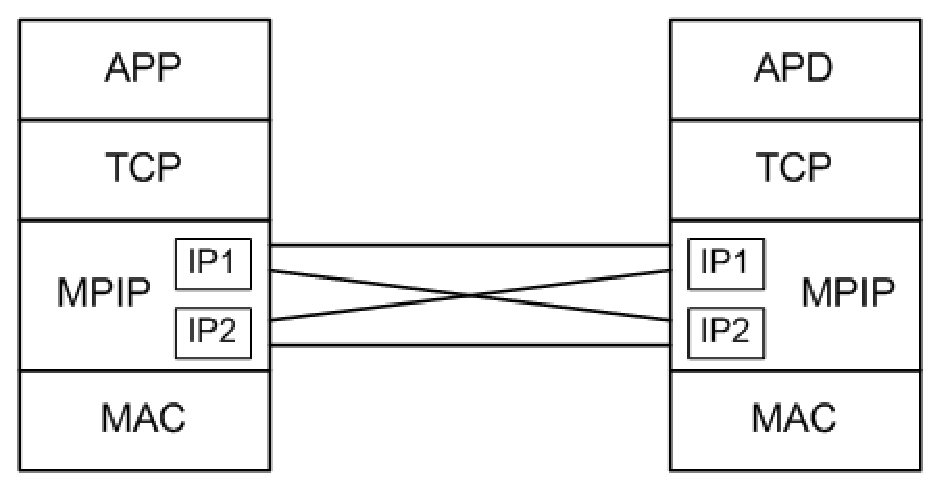
\includegraphics[width=1\linewidth]{fig/arch.eps}
%\caption{Work flow of sending and receiving a packet}
%\label{fig.flow}
%\end{figure}


\subsubsection{Dealing with out of order TCP traffic}

In modern devices, different interfaces can have totally different delay behaviour. For mobile devices, the WiFi interface and cellular interface can have huge difference in delay behaviour even if we connect them to the same service. Generally, cellular interface has much larger delay than WiFi; For PC devices, wired connection generally has smaller delay than WiFi interface. Under this situation, packets can be out of order frequently during the life time of a connection. This is not a problem for protocols like UDP, but for TCP, as shown below, packet out-of-order can result in catastrophic disaster for the overall performance.

In TCP Congestion Avoidance algorithm, a retransmission timer expiring or the reception of duplicate ACKs can implicitly signal the sender that a network congestion situation is occurring. The sender immediately sets its transmission window to one half of the current size. When a duplicate ACK is received, the sender does not know if it is because a TCP segment was lost or simply that a segment was delayed and received out of order at the receiver. If the receiver can re-order segments, it should not be long before the receiver sends the latest expected acknowledgement. Typically no more than one or two duplicate ACKs should be received when simple out of order conditions exist. If however more than two duplicate ACKs are received by the sender, it is a strong indication that at least one segment has been lost, the sender does not even wait for a retransmission timer to expire before retransmitting the segment and enter control avoidance stage, the sender\textquoteright s transmission window is cut off by one-half. This is the fast retransmit algorithm.

%(the minimum of the congestion window and the receiver's advertised window size), but to at least two segments. If congestion was indicated by a timeout, the congestion window is reset to one segment, which automatically puts the sender into Slow Start mode. If congestion was indicated by duplicate ACKs, the Fast Retransmit and Fast Recovery algorithms are invoked.

Considering multipath scenario, if the delay behaviour difference among different paths is not trivial, we can imagine a lot of out-of-order packets will happen. This will result in many fast retransmit events, even TCP can go back to slow start stage. Given that in modern Internet, real packet loss has become rare event, most of transmission window cut-off events are unnecessary at all. In our prototype, to solve the heterogeneous delay performance of different paths, we make specific process of TCP out-of-order packets. The overall process is shown in Figure~\ref{fig.outoforder}.

\begin{figure}
\centering
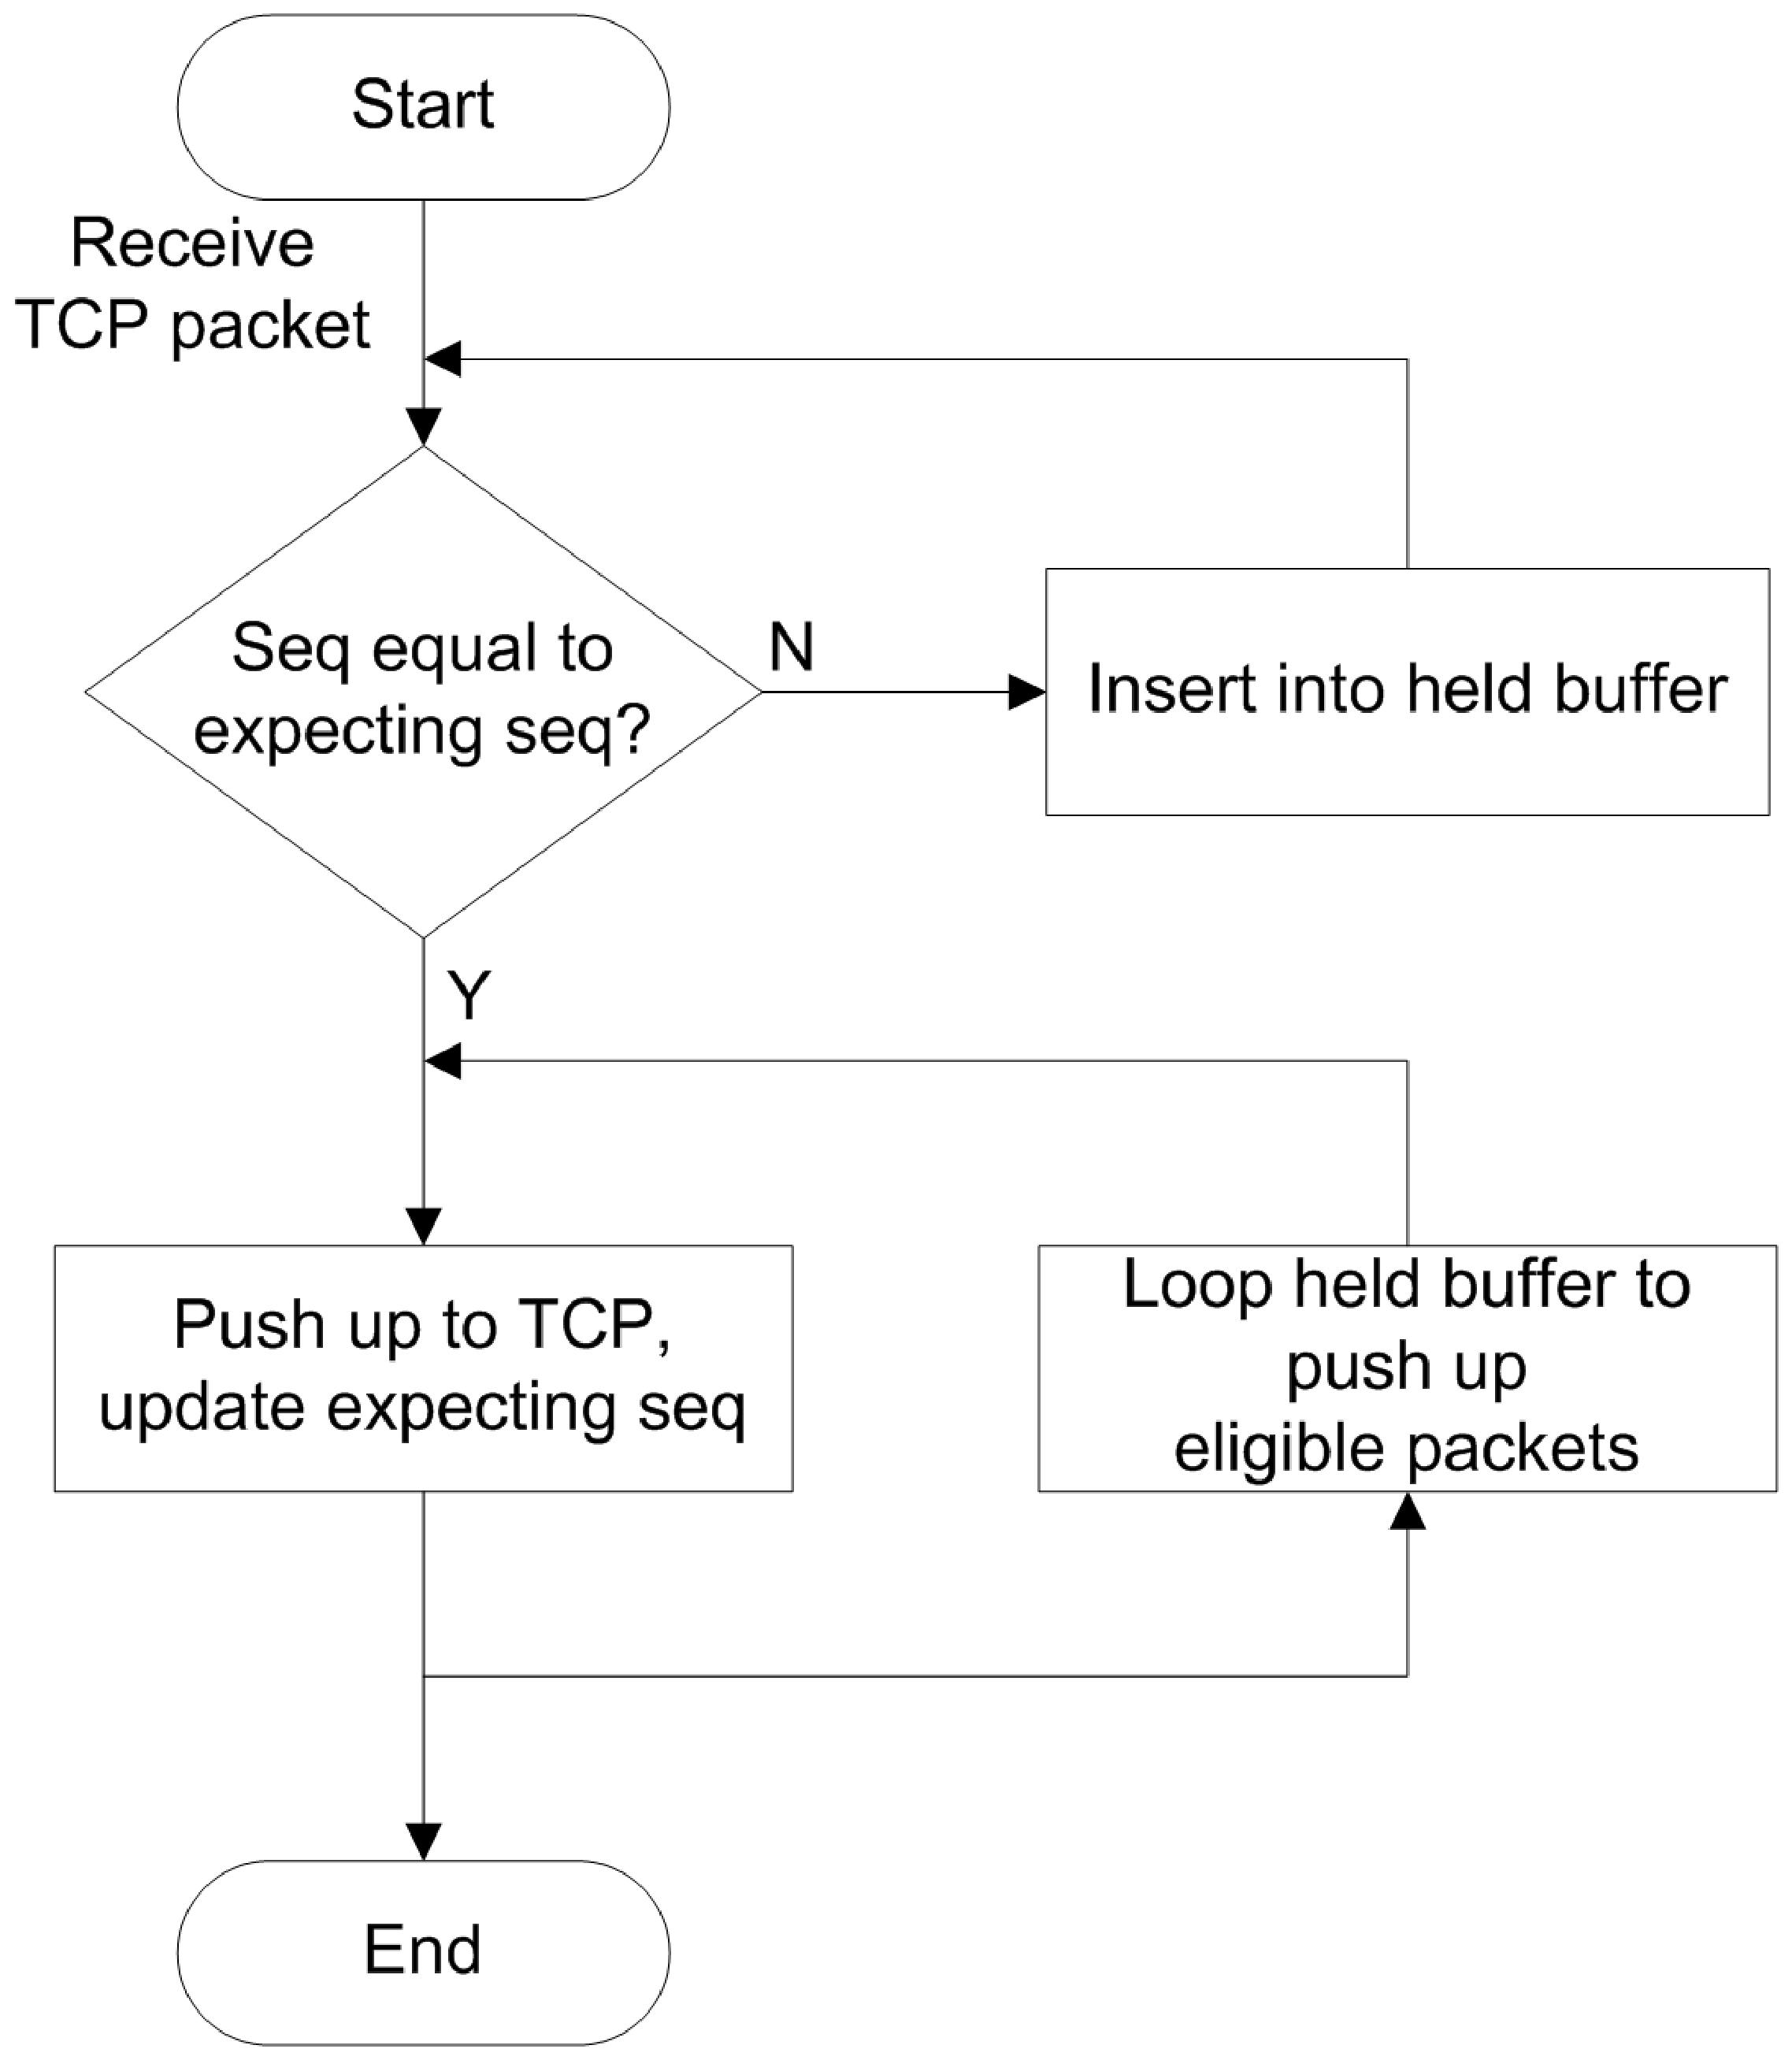
\includegraphics[width=0.8\linewidth]{fig/outoforder.eps}
\caption{TCP Out-Of-Order Packet Process}
\label{fig.outoforder}
\end{figure}


For each session in Table~\ref{tb.ss}, if it is TCP protocol, the system will maintain a buffer $B$ to store all out-of-order packets and the next expecting sequence number $S$. Every time one node receives a TCP packet, it takes out the sequence number, if it equals with the current expecting sequence number of the related session, the packet is pushed up to transportation layer immediately, and also, the buffered packets will be checked to see whether there are qualified packet for delivery. If not, the packet will be buffered into $B$ for future delivery. Every time one packet is pushed up to transportation layer, the next expecting sequence number $S$ of this session is updated through Equation~\ref{eq.seq} where $L$ is size of the whole packet, $H_{ip}$ is IP header size, and $H_{tcp}$ is TCP header size. TCP sequence number ranges from $0$ to $2^{32}-1$, Equation~\ref{eq.seq} can overflow $S$. But the data type of sequence number is unsigned integral, the number will loop back to $0$ automatically after that. 

\be
\label{eq.seq}
S(k) = S(k-1)+(L-H_{ip}-H_{tcp})
\ee

For the data structure that holds the TCP packets, a proper choice is to implement it as a binary tree, but according to our observations, most out-of-order packets come in an incremental order, and they are held at this step because of one late packet, when that late packet arrives, all the held packets will be pushed up. For this reason, we simply implement this structure a sorted list, every out-of-order packet will be inserted into this list according to its sequence number. The time complexity to insert this packet is almost $O(1)$ if we look up the list from the tail because most held packets arrive in an incremental order as mentioned.
When the expecting packet arrives, then all the waiting packets can be cleared from this list with a simple loop. This reduces code complexity greatly without sacrificing any performance.




\subsection{Andriod implementation}

%!TEX root =conext14.tex
\section{Performance Evaluation}
\label{sec:evaluation}
To evaluate the performance of our proposed system, we implemented our multipath IP in Ubuntu under Linux kernel $3.12.1$. Two desktops are installed with the MPIP enabled Ubuntu system. At each desktop, two NICs working at $25$Mbits/sec are installed which means that there are totally $4$ paths and the throughput upper bound is $50$Mbits/sec between the two nodes. We modify an open source software \bf{Simple Traffic Monitor}\cite{simon01} to record the real time traffic that goes through each NIC.

%For mobile devices, we implement this feature in Google Nexus $4$ with Android $4.01$.

\subsection{TCP/UDP throughput enhancement}
\label{sec:tcp}

In this section, we try to verify that our system can achieve high throughput in both TCP and UDP scenarios. As a typical implementation of multipath, MPTCP creates the highest TCP throughput record between two nodes in \cite{record}. In that demonstration, they used $6$ $1$Gbps NIC interfaces at each node, and connect them directly without only middle boxes, and they limited the number of paths to $6$ by setting up IP TABLES in Ubuntu. Also, they did bunch of TCP parameter optimization to squeeze out all possible throughout. They achieved a breathtaking $51$Gbps throughput in that demonstration. 

We don't have the same configuration of the record-breaking plat of MPTCP, but we use the same typical configuration for all scenarios to do side-by-side configuration. We try to verify that our implementation can achieve the same throughput improvement as MPTCP for TCP traffic, and also our system can have the same enhancement for UDP traffic. 

In our experiment setup, we have two PCs while each PC has two NIC cards, every NIC card works at 100Mbps. With these four NIC cards, we have different configurations to verify our system. For each configuration, we do side-by-side comparision among regular connection, MPTCP(For TCP), and MPIP connection. We use iperf to transmit traffic for five minutes, and we customized iperf to record real-time throughput of each second.

In Figure~\ref{fig.nonat}, we connect the two machine to the same router which means there are no NAT devices on all the paths.

\begin{figure*}[htb]
\centering{
\subfigure[TCP throughput with psudo TCP connection\label{fig.tcp_usetcp_nonat}]{\includegraphics[width=0.33\linewidth]{fig/tcp_usetcp_nonat.eps}}
\subfigure[TCP throughput with UDP Wrapper\label{fig.tcp_useudp_nonat}]{\includegraphics[width=0.33\linewidth]{fig/tcp_useudp_nonat.eps}}
\subfigure[UDP throughput\label{fig.udp_nonat}]{\includegraphics[width=0.33\linewidth]{fig/udp_nonat.eps}}
}
\caption{Side-by-side comparison without NAT}
\label{fig.nonat}
\end{figure*}

Also, we set up a NAT network with two routers as shown in Figure~\ref{fig.nat}. Because our router only has 100Mbps capacity while each NIC has 100Mbps, this means that our router can't fit all capacity of the NIC cards. To avoid this problem, we limit the bandwidth of our NIC cards to be 5Mbps with WonderShaper. Then the total capacity of our connection is 10Mbps. Figure~\ref{fig.nat} shows the result for this configuration.

\begin{figure*}[htb]
\centering{
\subfigure[TCP throughput with psudo TCP connection\label{fig.tcp_usetcp_nat}]{\includegraphics[width=0.33\linewidth]{fig/tcp_usetcp_nat.eps}}
\subfigure[TCP throughput with UDP Wrapper\label{fig.tcp_useudp_nat}]{\includegraphics[width=0.33\linewidth]{fig/tcp_useudp_nat.eps}}
\subfigure[UDP throughput\label{fig.udp_nat}]{\includegraphics[width=0.33\linewidth]{fig/udp_nat.eps}}
}
\caption{Side-by-side comparison with a simple NAT}
\label{fig.nat}
\end{figure*}


In Figure~\ref{fig.net}, we set up our server in Emulab to verify our system in Internet. Because the server in Emulab only has one public IP address which means our connection only has two paths. We do evaluation for both TCP and UDP. We can see that there is not throughput increase at all because the bottleneck is on the path of the connection. To improve throughput, we need another path that can avoid the bottleneck, like a $4$G path. Instead of increasing throughput, according to our evaluation, our MPIP implementation can perform as good as regular connection. And in TCP scenario, we reduce throughput fluctuations which happens a lot in regular TCP and MPTCP by using MPIP.

\begin{figure*}[htb]
\centering{
\subfigure[TCP throughput with psudo TCP connection\label{fig.tcp_usetcp_net}]{\includegraphics[width=0.33\linewidth]{fig/tcp_usetcp_net.eps}}
\subfigure[TCP throughput with UDP Wrapper\label{fig.tcp_useudp_net}]{\includegraphics[width=0.33\linewidth]{fig/tcp_useudp_net.eps}}
\subfigure[UDP throughput\label{fig.udp_net}]{\includegraphics[width=0.33\linewidth]{fig/udp_net.eps}}
}
\caption{Side-by-side comparison in Internet}
\label{fig.net}
\end{figure*}


\subsection{Skype voice call improvement}
\label{sec:skype}

In Figure~\ref{fig.skype}, we prove that our packet-size based routing decision works perfectly for audio application like Skype. In our experiment, we change the delay of NIC cards using the netem package in Ubuntu. On one side of the Skype call, we have two NIC cards as stated above. We ran the experiment for $360$ seconds with $3$ sections. In the first $120$ seconds, there is no manually added delay on each NIC card, we add additional $120ms$ delay to the first NIC card in the following $120$ seconds, finally for the last $120$ seconds, we add $120ms$ delay to the second NIC card. We did our Skype audio experiment without video content while most packets on the connection are audio packets except some control packets.The size of Audio packets is relative small, generally under $200$KB. In this case, according to Equation~\ref{eq.bw} to Equation~\ref{eq.c}, the routing decision will mostly depend on the delay value instead of queuing delay. Figure~\ref{fig.skype} shows the packets routing adaptation as the delay value changes. By this adaptation, we can make sure that the audio streaming will always choose the path that has lower delay to keep the best user experience even other paths have the same throughput.

\begin{figure}
\centering
\includegraphics[width=1\linewidth]{fig/skype.eps}
\caption{Skype Audio Streaming Routing Adaptation}
\label{fig.skype}
\end{figure}


\subsection{Smooth connection switch}
\label{sec:switch}

In Figure~\ref{fig.switch}, we verify that smooth switch between different NIC cards works perfectly over our MPIP implementation by doing an IPERF TCP experiment. We do a side-by-side comparison between MPIP and MPTCP. We also divide the experiment into $3$ sections with $120$ seconds for each section. On the client side of the connection, there are two NIC cards. In the first $120$ seconds, both NIC cards work synchronously, then we disable one of them for $120$ seconds, and during the last $120$ seconds, we enable back the NIC card. The result shows that our MPIP system can follow this on/off process perfectly with stable throughput. For MPTCP, as shown in previous experiments, MPTCP has higher fluctuation than MPIP even MPTCP can achieve higher throughput than MPIP. This happens because in MPTCP, there are more than one TCP connections ($4$ in this experiment), and each connection has its own congestion window. Although congestion control in MPTCP is coupled among different connections, fluctuation have more chances to happen with $4$ relatively independent congestion windows. But in MPIP, one one TCP connection is constructed for each session which means that there is only one congestion windows. In this case, the throughput is more consistent than that of MPTCP.

\begin{figure}
\centering
\includegraphics[width=1\linewidth]{fig/switch.eps}
\caption{Connection Smooth Switch}
\label{fig.switch}
\end{figure}


\subsection{Combination of MPIP and MPTCP}
\label{sec:mpip_mptcp}

MPTCP is implemented at Transportation Layer while MPIP is implemented at Network Layer. Both implementations try to be totally independent with other layers. Under this precondition, it is possible to combine MPTCP and MPIP together to see how the system performs. Based on the implementation of MPTCP V$0.88$, we merged our MPIP implementation to the source of MPTCP, and enable both MPTCP and MPIP.

In Figure~\ref{fig.mpip_mptcp}, we did an experiment of $20$ minutes to see how MPTCP, MPIP and combination of MPTCP and MPIP perform under the same network condition. As we can see, MPTCP can achieve much higher throughput than MPIP, but it doesn't stay there for long. The throughput fluctuates a lot through the whole experiment. On the other hand, when MPIP is applied, both MPIP alone and the combination of MPIP and MPTCP, consistent throughput can be achieved. Actually, MPIP alone has the best smoothness, but the combination also has huge improvement of consistency. The variance of each case can exactly reflect the difference. Table~\ref{tb.stat} shows the overall statistic result.

\begin{figure}
\centering
\includegraphics[width=1\linewidth]{fig/mpip_mptcp.eps}
\caption{Performance of MPIP, MPTCP and Combination}
\label{fig.mpip_mptcp}
\end{figure}

\begin{table}[htbp]
\caption{\label{tb.stat}MPIP, MPTCP, MPIP and MPTCP}
\centering
\begin{tabular}{|c|c|c|c|}
\hline
 & MPIP & MPTCP & MPIP and MPTCP\\
\hline
Variance (${10}^{12}$) & 2.65 & 417.08 & 14.46 \\
\hline
Average &&&\\
Throughput(Mbps) & 156.3 & 150.6 & 137.4  \\
\hline
\end{tabular}
\end{table}

%
%\subsection{Datacenter use case}
%\label{sec:datacenter}
%
%\subsection{Seamless handover with dynamic networks}
%\label{sec:handover}


\section{Conclusions and Future Work}
\label{sec:conclusion}

\bibliographystyle{./bib/IEEEtran}
\bibliography{./bib/IEEEfull}
\end{document}


